% !TEX TS-program = pdflatex
% !TEX encoding = UTF-8 Unicode
% !TEX ROOT = ../../main.tex

%Nutze nicht die automatische Nummerierung
%\renewcommand*\thesection*{}
%\renewcommand*\thesubsection*{}
%\renewcommand*\thesubsubsection*{}

%from https://github.com/ZaPF/Geschaeftsordnung_ZaPF
\section{Satzung der ZaPF}
\label{satzung}

\subsection*{§\,1 Name%
  \label{name}%
}

Die Tagung der Vertreterinnen und Vertreter der Physik-Fachschaften trägt den
Namen Zusammenkunft aller Physik-Fachschaften, kurz ZaPF.
Sie ist die Nachfolgeorganisation der Bundes-Fachschaften-Tagung Physik (BuFaTa Physik).


\subsection*{§\,2 Mitglieder%
  \label{mitglieder}%
}

Die ZaPF setzt sich aus Vertretern und Vertreterinnen und Mitgliedern der
Fachschaften Physik aller Hochschulen des deutschsprachigen Raumes zusammen.


\subsection*{§\,3 Aufgaben%
  \label{aufgaben}%
}

Die ZaPF findet einmal pro Semester statt und tagt öffentlich. Sie dient dem
Sammeln und der Diskussion von Informationen und tritt mit den Resultaten
gegebenenfalls an die Öffentlichkeit oder an Dritte heran.
Des Weiteren dient sie zum Gedanken- und Ideenaustausch zwischen den
Fachschaften.

Die ZaPF befasst sich mit studien- und hochschulrelevanten Themen. Sie besitzt
kein allgemeinpolitisches Mandat, kann sich jedoch in Bezug auf
hochschulpolitische Themen auch allgemeinpolitisch äußern. Hierbei muss ein
Zusammenhang zu studien- und hochschulpolitischen Belangen unmittelbar bestehen
und deutlich erkennbar bleiben.


\subsection*{§\,4 Tagung%
  \label{tagung}%
}

Die ausrichtende Fachschaft legt den Programmablauf der Tagung fest und
erarbeitet ein Protokoll der Veranstaltung, den sogenannten ZaPF-Reader. Sie
stellt davon allen Mitgliedsfachschaften ein Exemplar zur Verfügung.

Die Tagung beginnt mit dem Anfangsplenum und endet nach dem Abschlussplenum.


\subsection*{§\,5 Organe%
  \label{organe}%
}

Die Organe der ZaPF sind das ZaPF-Plenum, der Ständige Ausschuss der
Physik-Fachschaften (StAPF), die Vertrauenspersonen, das Kommunikationsgremium
(KomGrem) und der Technische Organisationsausschuss aller Physikfachschaften
(TOPF).

Die Wahlen von Mitgliedern des StAPF, des KomGrem und des TOPF sind
Personenwahlen entsprechend der Geschäftsordnung der ZaPF.

Die Mitgliedschaft im StAPF, dem Kommunikationsgremium oder dem TOPF endet mit
Ablauf der Amtszeit, Ableben des Amtsinhabers oder der Amtsinhaberin,
Niederlegung des Amtes oder Abwahl mit Zweidrittelmehrheit durch das Plenum. Der
Antrag auf Abwahl ist bis 15:00 Uhr am Vortag bei der ausrichtenden Fachschaft
anzukündigen.

Bis zur Nachwahl bleibt ein unbesetztes Amt vakant. Bei der Nachwahl wird das
Amt bis zum Ablauf der Restdauer der Amtszeit besetzt.
Die Nachwahl findet zum nächstmöglichen Zeitpunkt auf einem Abschlussplenum
einer Tagung statt.
Sollten nach einer Wahl Posten unbesetzt sein, bleiben sie vakant.

Falls mindestens zwei Drittel der Mitglieder eines Gremiums das Amt niederlegen,
gelten auch die Ämter der übrigen Mitglieder dieses Gremiums als vakant.


\subsubsection*{(a) Das ZaPF-Plenum%
  \label{a-das-zapf-plenum}%
}

Das ZaPF-Plenum ist das oberste beschlussfassende Gremium der ZaPF und setzt
sich aus allen Teilnehmerinnen und Teilnehmern der jeweiligen ZaPF zusammen.

Einzelne Themen werden in Arbeitskreisen diskutiert und für das Plenum vorbereitet.
Zu seinen Beschlusskompetenzen zählt auch die Wahl der Vertreter und Vertreterinnen
für den studentischen Akkreditierungspool für Bachelor- und Masterstudiengänge und
ähnliche Gremien.

Das Plenum beschließt ebenfalls die nächsten Veranstaltungsorte der ZaPF.

Den Ablauf der Plenen regelt die Geschäftsordnung für Plenen der ZaPF.


\subsubsection*{(b) Der Ständige Ausschuss der Physik-Fachschaften%
  \label{b-der-standige-ausschuss-der-physik-fachschaften}%
}

Der Ständige Ausschuss der Physik-Fachschaften (StAPF) vertritt die ZaPF in der
Öffentlichkeit.

Der StAPF besteht aus maximal fünf natürlichen Personen von mindestens drei
verschiedenen Hochschulen, welche für jeweils ein Jahr gewählt werden.

Die Amtszeit von drei Mitgliedern des StAPF beginnt zu einer im Sommersemester
stattfindenden ZaPF und die zweier StAPF-Mitglieder zu einer im Wintersemester
stattfindenden ZaPF.

Der StAPF konferiert öffentlich mindestens zweimal zwischen den ZaPFen.
Termin und Tagungsort (auf einer ZaPF, öffentlicher Chatraum, etc.) sind
rechtzeitig an geeigneter Stelle bekannt zu machen.

Der StAPF ist an die Weisungen des Plenums gebunden, kann jedoch
eigenverantwortlich handeln und muss seine Beschlüsse dem ZaPF-Plenum gegenüber
vertreten.
Die Entscheidungen innerhalb des StAPF müssen in diesen Fällen einstimmig fallen.
Der StAPF ist beschlussfähig falls mindestens drei seiner Mitglieder auf einer
Sitzung anwesend sind und der Beschluss in der Sitzungseinladung angekündigt
wurde.

Der StAPF gibt Informationen umgehend an die Fachschaften weiter.
Auf jeder ZaPF ist darüber hinaus ein Rechenschaftsbericht vorzulegen.

Der StAPF ist für die Archivierung und Veröffentlichung der Ergebnisse der ZaPF
verantwortlich, des Weiteren ist er Unterzeichner der ZaPF-Veröffentlichungen.
Der StAPF wählt sich aus seiner Mitte einen Sprecher.

Sollten alle Posten des StAPFes vakant sein, übernehmen die von der ZaPF
entsandten Mitglieder des Kommunikationsgremiums oder, falls diese vakant sind,
die Mitglieder des Technischen Organisationsausschuss aller Physikfachschaften
oder, falls auch diese vakant sind, die Mitglieder der letzten die ZaPF
ausrichtenden Fachschaft die Archivierungs- und Veröffentlichungsaufgaben des
StAPF.


\subsubsection*{(c) Die Vertrauenspersonen%
  \label{c-die-vertrauenspersonen}%
}

Die Vertrauenspersonen dienen als Anlaufstelle für hilfesuchende Personen, die
Ausgrenzung, Diskriminierung oder Belästigung im Rahmen der ZaPF erfahren haben.

Die Wahl der höchstens sechs Vertrauenspersonen ist zu Beginn jeder ZaPF durchzuführen.
Ihre Amtszeit endet mit dem Ende des Abschlussplenums oder Niederlegung des Amtes.

Die Wahl der Vertrauenspersonen ist in der Geschäftsordnung für Plenen der ZaPF
gesondert zu regeln.


\subsubsection*{(d) Das Kommunikationsgremium%
  \label{d-das-kommunikationsgremium}%
}

Das Kommunikationsgremium ist ein gemeinsames Gremium von ZaPF und jDPG.

Die Aufgaben dieses Gremiums sind der Austausch zwischen ZaPF und jDPG sowie
die Veröffentlichung gemeinsamer Beschlüsse.
Weiterhin entsendet dieses Gremium einen gemeinsamen Vertreter oder eine
gemeinsame Vertreterin zur KFP.

Die ZaPF entsendet zwei Mitglieder in das Kommunikationsgremium.

Davon beginnt die Amtszeit eines Mitgliedes auf einer ZaPF im Sommersemester und
die des anderen Mitgliedes auf einer ZaPF im Wintersemester.

Die Amtszeit der Mitglieder im Kommunikationsgremium beläuft sich auf ein Jahr.

Näheres regelt das Dokument zur \textquotedbl{}Regelung zur Zusammenarbeit von jDPG und ZaPF
in hochschulpolitischen Fragestellungen\textquotedbl{} in der Fassung vom Endplenum der ZaPF
im Sommersemester 2010 in Frankfurt.


\subsubsection*{(e) Der Technische Organisationsausschuss aller Physikfachschaften (TOPF)%
  \label{e-der-technische-organisationsausschuss-aller-physikfachschaften-topf}%
}

Der Technische Organisationsausschuss aller Physikfachschaften (TOPF) ist für
die Instandhaltung und Dokumentation der EDV-Projekte der ZaPF verantwortlich.

Er besteht aus zwei vom Plenum zu bestimmenden Personen, die für die
Aufrechterhaltung des Betriebs und die Dokumentation der Basissysteme
hauptverantwortlich sind, und einer beliebigen Anzahl von freiwilligen Helfern,
die für die Dokumentation und den Betrieb von einzelnen Projekten verantwortlich
sind.

Die Hauptverantwortlichen sind dem Plenum und dem StAPF rechenschaftspflichtig
und an ihre Weisungen gebunden. Insbesondere hat das Plenum die Möglichkeit,
Datenschutzerklärungen und Nutzungsordnungen sowohl für das Gesamtsystem als
auch für einzelne Projekte zu bestimmen.

Die freiwilligen Helfer werden nicht gewählt, sondern durch die beiden
Hauptverantwortlichen gemeinsam bestimmt. Sie sind ihnen rechenschaftspflichtig
sowie an deren Weisungen und die erlassenen Ordnungen gebunden.

Die Amtszeit eines Hauptverantwortlichen beginnt zu einer im Sommersemester
stattfindenden ZaPF, die des anderen zu einer im Wintersemester stattfindenden
ZaPF.

Die Amtszeit der Hauptverantwortlichen beträgt ein Jahr.


\subsection*{§\,6 Satzungsänderungen%
  \label{satzungsanderungen}%
}

Änderungen dieser Satzung benötigen eine Zweidrittelmehrheit, wobei Beschlussfähigkeit
des Plenums vor der Abstimmung zwingend festzustellen ist. Satzungsänderungen
sind nicht durch Initiativanträge möglich und können nur auf dem Endplenum
abgestimmt werden.

Wünsche nach einer Satzungsänderung sind bis spätestens sieben Tage vor dem
Anfangsplenum geeignet (z.B. über die ZaPF-Mailingliste)
zusammen mit einem Antragsentwurf oder mindestens einer schriftlichen
Begründung und einem konkreten Thema der Satzungsänderung anzukündigen.

Auf der ZaPF muss dann zwingend ein Arbeitskreis zum Thema der vorgeschlagenen
Satzungsänderungen durchgeführt werden, dessen Satzungsänderungsantrag bzw.
Satzungsänderungsanträge bis spätestens 15:00 Uhr am Vortag des Endplenums bei
der die ZaPF ausrichtenden Fachschaft eingereicht und ausgehängt werden müssen.


\subsection*{Schlussbestimmungen und Änderungshistorie%
  \label{schlussbestimmungen-und-anderungshistorie}%
}

Die vorliegende Satzung wurde anlässlich der ZaPF '06 in Dresden vorbereitet,
mit einer Zweidrittelmehrheit der anwesenden Fachschaften beschlossen und
angenommen. Diese Satzung setzt alle bisherigen außer Kraft. Sie trat zum
28.05.2006 in Kraft.

Inhaltliche Änderungen wurden vorgenommen auf der:
%
\begin{itemize}

\item Sommer-ZaPF 2007 in Berlin,

\item Sommer-ZaPF 2008 in Konstanz,

\item Sommer-ZaPF 2009 in Göttingen,

\item Sommer-ZaPF 2011 in Dresden,

\item Sommer-ZaPF 2013 in Jena,

\item Sommer-ZaPF 2014 in Düsseldorf,

\item Winter-ZaPF 2014 in Bremen,

\item Sommer-ZaPF 2015 in Aachen,

\item Winter-ZaPF 2015 in Frankfurt am Main,

\item Sommer-ZaPF 2016 in Konstanz,

\item und auf der Sommer-ZaPF 2017 in Berlin.

\end{itemize}

\begin{figure}[b]
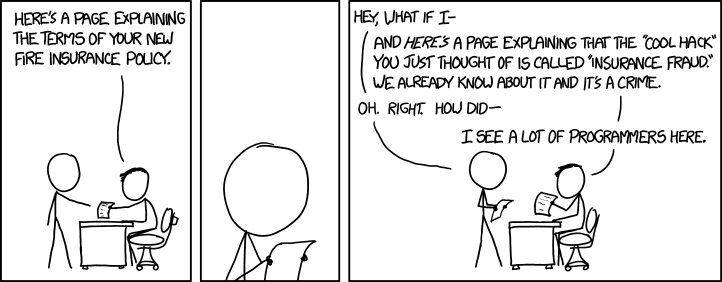
\includegraphics[width=\textwidth]{insurance}
\end{figure}